%==============================================================================
%  LAB REPORT 6 — IMU Sensor Data Reading for Inertial Navigation
%  Compile with pdfLaTeX (works out of the box on Overleaf).
%
%  >>> PASTE YOUR GOOGLE DRIVE LINKS IN THE MACROS MARKED "EDIT ME" BELOW <<<
%==============================================================================
\documentclass[10pt,a4paper]{article}

%---------------------------------------- page geometry
\usepackage[a4paper,top=2.2cm,bottom=2.0cm,left=2.1cm,right=2.1cm,
            headsep=13pt,footskip=22pt]{geometry}

%---------------------------------------- encoding & fonts
\usepackage[T1]{fontenc}
\usepackage[utf8]{inputenc}
\usepackage{newtxtext,newtxmath}     % Times-like professional text + math
\usepackage[scaled=0.86]{beramono}   % clean monospace for code
\usepackage{microtype}

%---------------------------------------- graphics, colour, boxes
\usepackage{graphicx}
\usepackage[dvipsnames,table]{xcolor}
\usepackage{tikz}
\usepackage{circuitikz}
\usepackage{pgfplots}
\pgfplotsset{compat=1.18}
\usepgfplotslibrary{groupplots}
\usepackage[most]{tcolorbox}
\usepackage{booktabs}
\usepackage{array}
\usepackage{tabularx}
\usepackage{enumitem}
\usepackage{listings}
\usepackage{fancyhdr}
\usepackage{titlesec}
\usepackage{caption}
\usepackage{float}
\usepackage{needspace}
\usetikzlibrary{arrows.meta,positioning,calc,shadows.blur,decorations.pathreplacing}
\ctikzset{bipoles/length=0.62cm}   % compact component symbols

%---------------------------------------- hyperlinks (load late)
\usepackage[hidelinks]{hyperref}
\usepackage{url}
% print a URL stored in a macro, safely (handles _ ~ % etc.)
\newcommand{\showurl}[1]{\expandafter\url\expandafter{#1}}

%==============================================================================
%  Student details
%==============================================================================
\newcommand{\studentname}{Chavan Atharva Sunil}
\newcommand{\rollnumber}{240003021}
\newcommand{\coursecode}{AA303 --- IoT for Space Applications}
\newcommand{\expdate}{10 September 2026 (ESP32) and 20 September 2026 (Raspberry Pi)}

%  Google Drive folder holding the demonstration videos and the source code
\urldef{\drivefolder}\url{https://drive.google.com/drive/folders/1cdR2mrryf5j0LEnQgIgYEAs-zB0Qj0jO?usp=sharing}

%==============================================================================
%  Colour palette
%==============================================================================
\definecolor{ink}{HTML}{1B2733}      % body text / headings
\definecolor{accent}{HTML}{0B5FA5}   % primary blue
\definecolor{accentlt}{HTML}{E8F1FA} % pale blue fill
\definecolor{amber}{HTML}{C8791A}    % LED amber
\definecolor{amberlt}{HTML}{FDF3E3}
\definecolor{rule}{HTML}{C9D4DE}
\definecolor{soft}{HTML}{F5F7F9}
\definecolor{codebg}{HTML}{F7F9FB}
\definecolor{cmnt}{HTML}{6C8090}
\definecolor{kw}{HTML}{0B5FA5}
\definecolor{str}{HTML}{1C7C54}
\definecolor{num}{HTML}{9B2D5E}

\color{ink}

%==============================================================================
%  Headings
%==============================================================================
\titleformat{\section}
  {\normalfont\large\bfseries\color{accent}}
  {\raisebox{0pt}{\colorbox{accent}{\color{white}\bfseries\;\thesection\;}}}
  {0.7em}{}[\vspace{2pt}{\color{rule}\titlerule[0.8pt]}]
\titlespacing*{\section}{0pt}{14pt}{8pt}

\titleformat{\subsection}
  {\normalfont\normalsize\bfseries\color{ink}}{\thesubsection}{0.6em}{}
\titlespacing*{\subsection}{0pt}{11pt}{4pt}

\titleformat{\subsubsection}
  {\normalfont\small\bfseries\color{accent}}{}{0em}{}
\titlespacing*{\subsubsection}{0pt}{9pt}{2pt}

%==============================================================================
%  Header / footer
%==============================================================================
\pagestyle{fancy}
\fancyhf{}
\renewcommand{\headrulewidth}{0.4pt}
\renewcommand{\footrulewidth}{0pt}
\fancyhead[L]{\footnotesize\color{cmnt}\textsc{Lab Report 6} \,\textbar\, IMU Sensor Data Reading for Inertial Navigation}
\fancyhead[R]{\footnotesize\color{cmnt}\studentname\ \,\textbar\, \rollnumber}
\fancyfoot[C]{\footnotesize\color{cmnt}\thepage}

%==============================================================================
%  Captions & lists
%==============================================================================
\captionsetup{font=small,labelfont={bf,color=accent},skip=6pt}
\setlist[itemize]{leftmargin=1.35em,itemsep=2pt,topsep=3pt}
\setlist[enumerate]{leftmargin=1.6em,itemsep=2.5pt,topsep=3pt}
\renewcommand{\arraystretch}{1.18}

%==============================================================================
%  Custom boxes
%==============================================================================
\newtcolorbox{keybox}[1][]{
  enhanced, breakable, colback=accentlt, colframe=accent,
  boxrule=0pt, leftrule=3pt, arc=2pt, left=10pt, right=10pt, top=8pt, bottom=8pt,
  fontupper=\normalsize, #1}

\newtcolorbox{notebox}[1][]{
  enhanced, breakable, colback=amberlt, colframe=amber,
  boxrule=0pt, leftrule=3pt, arc=2pt, left=10pt, right=10pt, top=7pt, bottom=7pt,
  fontupper=\small, #1}

\newtcolorbox{titledbox}[2][]{
  enhanced, breakable, colback=white, colframe=rule, boxrule=0.6pt, arc=3pt,
  left=10pt, right=10pt, top=8pt, bottom=8pt,
  title={\bfseries\small #2}, coltitle=white, colbacktitle=accent,
  attach boxed title to top left={xshift=8pt,yshift=-8pt},
  boxed title style={boxrule=0pt,arc=2pt,left=6pt,right=6pt,top=2pt,bottom=2pt},
  #1}

%==============================================================================
%  Code listing style
%==============================================================================
\lstdefinestyle{prostyle}{
  backgroundcolor=\color{codebg},
  basicstyle=\ttfamily\scriptsize\color{ink},
  keywordstyle=\color{kw}\bfseries,
  commentstyle=\color{cmnt}\itshape,
  stringstyle=\color{str},
  numberstyle=\ttfamily\tiny\color{cmnt},
  numbers=left, numbersep=9pt, xleftmargin=17pt, xrightmargin=2pt,
  frame=single, framesep=6pt, rulecolor=\color{rule},
  breaklines=true, showstringspaces=false, tabsize=2,
  columns=fullflexible, keepspaces=true,
  aboveskip=8pt, belowskip=6pt,
  emphstyle=\color{num}\bfseries,
  literate={°}{{$^{\circ}$}}1
}
\lstset{style=prostyle}

%==============================================================================
%  Schematic: I2C connection from a board's header to the GY-521 (MPU6050)
%  \imuschematic{board}{vcc pin}{sda pin}{scl pin}{gnd pin}
%==============================================================================
\newcommand{\imuschematic}[5]{%
\begin{circuitikz}[scale=0.71, transform shape, every node/.style={font=\footnotesize}]
  \draw[fill=accentlt, draw=accent, line width=0.9pt, rounded corners=4pt]
        (-3.5,-0.45) rectangle (-0.6,4.15);
  \node[text=accent, font=\small\bfseries] at (-2.05,3.65) {#1};
  \node[text=cmnt,   font=\scriptsize]     at (-2.05,3.25) {I$^2$C master};
  \foreach \y/\pin/\name in {2.55/#2/3.3\,V, 1.75/#3/SDA, 0.95/#4/SCL, 0.15/#5/GND}{
     \draw[fill=white, draw=accent, line width=0.6pt] (-0.92,\y-0.14) rectangle (-0.6,\y+0.14);
     \node[anchor=east, font=\scriptsize\bfseries, text=accent, align=right] at (-1.02,\y) {\pin\\[-2pt]{\tiny\color{cmnt}\name}};}
  \draw[line width=1.1pt, red!70!black] (-0.6,2.55) -- (3.0,2.55);
  \draw[line width=1.1pt, green!50!black] (-0.6,1.75) -- (3.0,1.75);
  \draw[line width=1.1pt, yellow!70!black] (-0.6,0.95) -- (3.0,0.95);
  \draw[line width=1.1pt, black]        (-0.6,0.15) -- (3.0,0.15);
  \node[font=\tiny, text=red!70!black, anchor=south] at (1.2,2.6)  {VCC};
  \node[font=\tiny, text=green!40!black, anchor=south] at (1.2,1.8) {SDA --- data};
  \node[font=\tiny, text=yellow!50!black, anchor=south] at (1.2,1.0) {SCL --- clock};
  \node[font=\tiny, text=cmnt, anchor=south] at (1.2,0.2) {GND};
  \draw[fill=soft, draw=rule, line width=0.8pt, rounded corners=4pt] (3.0,-0.45) rectangle (7.9,4.15);
  \node[text=ink, font=\small\bfseries] at (5.45,3.7) {GY-521 module};
  \node[text=cmnt, font=\scriptsize] at (5.45,3.33) {MPU6050 breakout, I$^2$C};
  \foreach \y/\lab in {2.55/VCC, 1.75/SDA, 0.95/SCL, 0.15/GND}{
     \draw[fill=white, draw=ink, line width=0.6pt] (3.0,\y-0.14) rectangle (3.32,\y+0.14);
     \node[anchor=west, font=\tiny\bfseries] at (3.34,\y) {\lab};}
  \draw[line width=0.7pt] (3.32,2.55) -- (4.3,2.55);
  \draw[line width=0.7pt] (4.3,2.55) -- (4.3,2.45) to[R, l_=$2.2\,\mathrm{k}\Omega$] (4.3,1.75);
  \draw[line width=0.7pt] (4.3,2.55) -- (5.0,2.55) -- (5.0,2.45) to[R] (5.0,0.95);
  \draw[line width=0.7pt] (3.32,1.75) -- (4.3,1.75) -- (6.2,1.75);
  \draw[line width=0.7pt] (3.32,0.95) -- (5.0,0.95) -- (6.2,0.95);
  \draw[line width=0.7pt] (5.0,2.55) -- (6.2,2.55);
  \draw[line width=0.7pt] (3.32,0.15) -- (6.2,0.15);
  \fill (4.3,2.55) circle (1.2pt); \fill (5.0,2.55) circle (1.2pt);
  \fill (4.3,1.75) circle (1.2pt); \fill (5.0,0.95) circle (1.2pt);
  \draw[fill=cyan!20, draw=cyan!60!black, line width=0.8pt] (6.2,-0.2) rectangle (7.7,2.95);
  \node[font=\scriptsize\bfseries, text=cyan!40!black, rotate=90] at (7.35,1.4) {MPU6050};
  \node[font=\tiny, anchor=west] at (6.22,2.72) {VDD};
  \node[font=\tiny, anchor=west] at (6.22,1.92) {SDA};
  \node[font=\tiny, anchor=west] at (6.22,1.12) {SCL};
  \node[font=\tiny, anchor=west] at (6.22,0.32) {GND};
  \node[font=\tiny, text=cmnt, anchor=north] at (5.45,-0.5) {AD0 pulled LOW on the module $\Rightarrow$ address 0x68};
\end{circuitikz}}

%==============================================================================
\begin{document}

%------------------------------------------------------------------ TITLE BLOCK
\thispagestyle{empty}
\begin{tikzpicture}[remember picture, overlay]
  \fill[accent] (current page.north west) rectangle
        ($(current page.north east)+(0,-7.15cm)$);
  \fill[amber] ($(current page.north west)+(0,-7.15cm)$) rectangle
        ($(current page.north east)+(0,-7.3cm)$);
\end{tikzpicture}

\vspace*{0.35cm}
{\color{white}
 \noindent{\footnotesize\textsc{\coursecode}}\\[2pt]
 \noindent{\Large\bfseries Experiment 6 \,\textbar\, Lab Report}\\[8pt]
 \noindent{\huge\bfseries IMU Sensor Data Reading}\\[6pt]
 \noindent{\LARGE\bfseries for Inertial Navigation: Acceleration and Angular Velocity}\\[10pt]
 \noindent{\small Reading a six-axis MPU6050 inertial measurement unit over I$^2$C on a Raspberry Pi, and publishing it from an ESP32 as a live web dashboard}
}
\vspace{1.5cm}

\noindent
\begin{tabularx}{\textwidth}{@{}>{\bfseries\color{accent}}l X@{}}
\toprule
Submitted by  & \studentname \\
Roll Number   & \rollnumber \\
Date of Experiment & \expdate \\
Boards Used   & Raspberry Pi 4 (I$^2$C bus 1, GPIO2/GPIO3) and ESP32 DevKit (I$^2$C on GPIO21/GPIO22) \\
\bottomrule
\end{tabularx}

\vspace{10pt}

%------------------------------------------------------------------ 1. AIM
\section{Aim}

\begin{keybox}
To read the three-axis \textbf{acceleration} and three-axis \textbf{angular velocity}
of an \textbf{MPU6050} inertial measurement unit (IMU) over the I$^2$C bus, and to
relate these six quantities to what an inertial navigation system needs: the
specific force from which velocity and position are integrated, and the turn rate
from which orientation is tracked. The IMU is read first from a \textbf{Raspberry Pi},
printing the values to the terminal, and then from an \textbf{ESP32}, which serves them
as a live web dashboard on its own Wi-Fi network while the sensor is moved by hand.
\end{keybox}

\subsection*{Objectives}
\begin{itemize}
  \item To connect a GY-521 (MPU6050) breakout to a Raspberry Pi and to an ESP32 over
        the two-wire I$^2$C bus and identify it at its address \texttt{0x68}.
  \item To read the accelerometer, gyroscope and temperature registers through a driver
        library on each board, in physical units ($g$, $^{\circ}$/s, $^{\circ}$C).
  \item To verify the readings against physics: at rest the acceleration vector has
        magnitude $1\,g$ (gravity) and the gyroscope reads zero; when the sensor is
        tilted the $1\,g$ redistributes between the axes, and when it is turned the
        gyroscope shows the rate of turn.
  \item To display the six values live in a browser served by the ESP32, and to discuss
        how they would be integrated into velocity, position and orientation --- and why
        that integration drifts.
\end{itemize}

\subsection*{Brief Theory}
An \emph{inertial measurement unit} combines an accelerometer and a gyroscope, each
with three orthogonal axes. The MPU6050 is a MEMS device: microscopic proof masses on
silicon springs move under acceleration, and vibrating structures are deflected by the
Coriolis force when the chip rotates; both displacements are read capacitively and
digitised by 16-bit ADCs. The accelerometer full scale is selectable from $\pm2$ to
$\pm16\,g$ and the gyroscope from $\pm250$ to $\pm2000\,^{\circ}$/s; the defaults used
here, $\pm2\,g$ and $\pm250\,^{\circ}$/s, give resolutions of $61\,\mu g$ and
$0.0076\,^{\circ}$/s per count. A temperature sensor is included for compensation.

\subsubsection{What the two sensors measure}
The accelerometer does \emph{not} measure the acceleration of the sensor directly. It
measures the \emph{specific force} $\mathbf{f} = \mathbf{a} - \mathbf{g}$: the sum of
the sensor's own acceleration and the reaction to gravity. A sensor lying still on a
table therefore reads $+1\,g$ on the axis pointing up and zero on the other two, and
the magnitude
\[
  |\mathbf{f}| = \sqrt{a_x^2 + a_y^2 + a_z^2}
\]
is $1\,g$ in \emph{any} orientation as long as the sensor is not accelerating. Tilting
the sensor merely redistributes that $1\,g$ between the axes, which is what makes the
accelerometer a tilt sensor:
\[
  \text{pitch} = \arctan\frac{a_x}{\sqrt{a_y^2 + a_z^2}},\qquad
  \text{roll}  = \arctan\frac{a_y}{\sqrt{a_x^2 + a_z^2}} .
\]
The gyroscope measures angular velocity $\boldsymbol{\omega}$ about each axis in
$^{\circ}$/s: zero when the sensor is still, whatever its orientation, and non-zero only
while it is turning.

\subsubsection{From IMU readings to navigation}
Inertial navigation is the process of integrating these six quantities:
\[
  \boldsymbol{\theta}(t) = \int \boldsymbol{\omega}\,dt,\qquad
  \mathbf{v}(t) = \int \bigl(R(\boldsymbol{\theta})\,\mathbf{f} + \mathbf{g}\bigr)\,dt,\qquad
  \mathbf{p}(t) = \int \mathbf{v}\,dt .
\]
The gyroscope is integrated once to track the orientation $\boldsymbol{\theta}$; that
orientation is used to rotate the specific force into the world frame and remove
gravity; the result is integrated once for velocity and again for position. Every
integration also integrates the sensor's errors --- a constant gyro bias becomes a
steadily growing angle error, and an accelerometer bias of only $1\,\mathrm{m}g$ becomes
a position error growing as $\tfrac12 b t^2$, about $18\,\mathrm{m}$ after one minute
--- so an IMU alone is only useful for short intervals and is always combined with an
absolute reference (GPS, a barometer, a magnetometer, star trackers on a spacecraft)
that resets the drift.

\begin{figure}[htb]
\centering
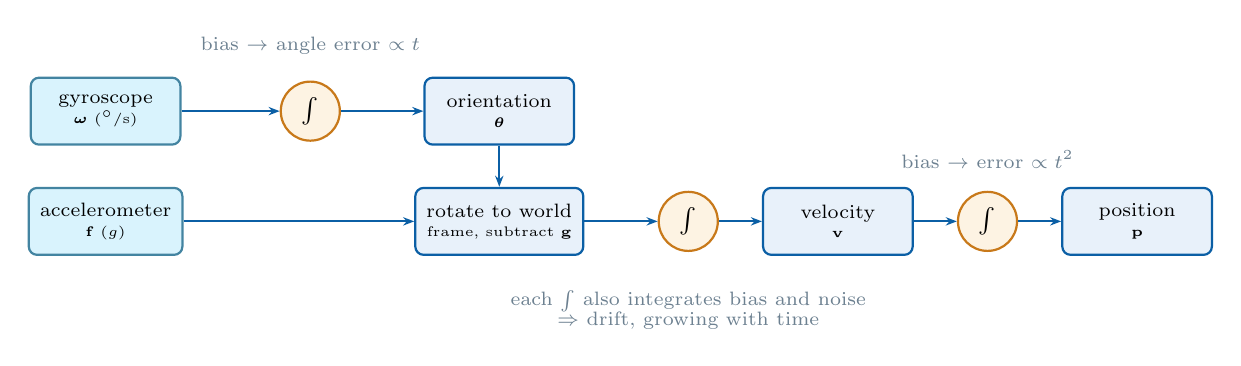
\begin{tikzpicture}[x=1cm, y=1cm, every node/.style={font=\scriptsize}]
  \tikzset{blk/.style={draw=accent, fill=accentlt, line width=0.8pt, rounded corners=3pt,
                       minimum height=0.85cm, minimum width=1.9cm, align=center, inner sep=4pt}}
  \tikzset{op/.style={draw=amber, fill=amberlt, line width=0.8pt, circle, minimum size=0.75cm, inner sep=1pt, font=\small}}
  \node[blk, fill=cyan!15, draw=cyan!60!black] (gy) at (0,1.4) {gyroscope\\[-1pt]{\tiny $\boldsymbol\omega$ ($^{\circ}$/s)}};
  \node[blk, fill=cyan!15, draw=cyan!60!black] (ac) at (0,0) {accelerometer\\[-1pt]{\tiny $\mathbf f$ ($g$)}};
  \node[op] (i1) at (2.6,1.4) {$\int$};
  \node[blk] (th) at (5.0,1.4) {orientation\\[-1pt]{\tiny $\boldsymbol\theta$}};
  \node[blk] (rot) at (5.0,0) {rotate to world\\[-1pt]{\tiny frame, subtract $\mathbf g$}};
  \node[op] (i2) at (7.4,0) {$\int$};
  \node[blk] (v) at (9.3,0) {velocity\\[-1pt]{\tiny $\mathbf v$}};
  \node[op] (i3) at (11.2,0) {$\int$};
  \node[blk] (p) at (13.1,0) {position\\[-1pt]{\tiny $\mathbf p$}};
  \draw[-{Stealth[length=4pt]}, accent, line width=0.8pt] (gy) -- (i1);
  \draw[-{Stealth[length=4pt]}, accent, line width=0.8pt] (i1) -- (th);
  \draw[-{Stealth[length=4pt]}, accent, line width=0.8pt] (th) -- (rot);
  \draw[-{Stealth[length=4pt]}, accent, line width=0.8pt] (ac) -- (rot);
  \draw[-{Stealth[length=4pt]}, accent, line width=0.8pt] (rot) -- (i2);
  \draw[-{Stealth[length=4pt]}, accent, line width=0.8pt] (i2) -- (v);
  \draw[-{Stealth[length=4pt]}, accent, line width=0.8pt] (v) -- (i3);
  \draw[-{Stealth[length=4pt]}, accent, line width=0.8pt] (i3) -- (p);
  \node[text=cmnt, anchor=north, align=center] at (7.4,-0.75) {each $\int$ also integrates bias and noise\\[-1pt]$\Rightarrow$ drift, growing with time};
  \node[text=cmnt, anchor=south] at (2.6,2.0) {bias $\to$ angle error $\propto t$};
  \node[text=cmnt, anchor=south] at (11.2,0.55) {bias $\to$ error $\propto t^2$};
\end{tikzpicture}
\caption{The inertial-navigation chain. This experiment produces the two inputs on the
left; the discussion returns to why the integrations on the right drift.}
\label{fig:ins}
\end{figure}

\begin{notebox}
\textbf{The module.} The sensor came as a \textbf{GY-521} breakout: the MPU6050 with its
own $3.3\,\mathrm{V}$ regulator (so VCC accepts $3.3$ or $5\,\mathrm{V}$), pull-up
resistors on SDA and SCL, and the AD0 address pin pulled LOW, which sets the I$^2$C
address to \texttt{0x68}. Only four of its eight pins are needed: VCC, GND, SDA and
SCL. The bus pins are the same ones as in Experiment~5 --- GPIO2/GPIO3 on the Raspberry
Pi (I$^2$C must be enabled) and GPIO21/GPIO22 on the ESP32.
\end{notebox}

%------------------------------------------------------------------ 2. MATERIALS
\Needspace{8\baselineskip}
\section{Materials Required}

\noindent
\begin{tabularx}{\textwidth}{@{}p{0.4cm} >{\raggedright\arraybackslash}p{5.6cm} c X@{}}
\toprule
\rowcolor{soft}
\multicolumn{1}{@{}l}{\textbf{\#}} & \textbf{Component} & \textbf{Qty.} & \textbf{Purpose in the setup} \\
\midrule
1 & Raspberry Pi 4 (in case, with SD card, OS installed) & 1 & Part A host; I$^2$C master, prints readings to the terminal (also powers the ESP32 over USB in Part B) \\
2 & ESP32 DevKit (30-pin)                                 & 1 & Part B host; I$^2$C master, Wi-Fi access point and web server \\
3 & GY-521 breakout with MPU6050 (6-axis IMU)             & 1 & Measures acceleration and angular velocity; shared between the two parts \\
4 & Female--female jumper wires                            & 4 & VCC, GND, SDA and SCL between header and module \\
5 & Micro-USB cable, laptop with Arduino IDE, and a tablet or phone with Wi-Fi & 1 & Programming the ESP32 and viewing the dashboard \\
6 & USB-C power supply, monitor, keyboard and mouse        & 1 & Running and observing the Raspberry Pi \\
7 & Software: \texttt{smbus2} (Pi); \texttt{Adafruit MPU6050} library and ESP32 core (Arduino IDE) & --- & I$^2$C access on the Pi; sensor driver on the ESP32 \\
\bottomrule
\end{tabularx}

%------------------------------------------------------------------ 3. METHODOLOGY
\section{Methodology}

The same GY-521 module was used on both boards, wired the same way each time: four
jumper wires for VCC, GND, SDA and SCL. The module's other pins (XDA, XCL, AD0, INT)
were left unconnected, which leaves it in plain I$^2$C mode at \texttt{0x68}. No
breadboard or extra components were needed because the pull-up resistors and the
regulator are on the module.

\subsection{Connections}

\vspace{2pt}
\noindent
\begin{tabularx}{\textwidth}{@{}l l l >{\raggedright\arraybackslash}X@{}}
\toprule
\rowcolor{soft}
\textbf{Module pin} & \textbf{Raspberry Pi 4 (Part A)} & \textbf{ESP32 (Part B)} & \textbf{Function} \\
\midrule
VCC & Pin 1 --- $3.3\,\mathrm{V}$ & 3V3 (red)            & Supply, through the module's regulator \\
GND & Pin 6 --- GND               & GND (black)          & Ground \\
SDA & Pin 3 --- GPIO2 (SDA1) & GPIO21 (green) & Serial data, bidirectional \\
SCL & Pin 5 --- GPIO3 (SCL1) & GPIO22 (yellow) & Serial clock from the master \\
XDA, XCL, AD0, INT & not connected & not connected & Auxiliary bus, address select (LOW $\Rightarrow$ \texttt{0x68}), interrupt \\
\bottomrule
\end{tabularx}

\begin{figure}[htb]
\centering
\begin{minipage}[t]{0.49\textwidth}
\centering
\imuschematic{Raspberry Pi}{Pin 1}{Pin 3}{Pin 5}{Pin 6}
\end{minipage}\hfill
\begin{minipage}[t]{0.49\textwidth}
\centering
\imuschematic{ESP32}{3V3}{GPIO21}{GPIO22}{GND}
\end{minipage}
\caption{Circuit schematics for the two parts. Four wires each; the pull-ups and the
address-setting AD0 resistor are on the GY-521 module. Wire colours as used in Part B.}
\label{fig:schematic}
\end{figure}

\subsection{Part A --- Raspberry Pi, readings on the terminal}

With I$^2$C enabled, the sensor was confirmed on the bus with \texttt{i2cdetect -y 1}
and the \texttt{smbus2} library installed:

\begin{lstlisting}[language=bash, caption={Preparing the Raspberry Pi.}, label={lst:install}]
sudo raspi-config          # Interface Options -> I2C -> Enable
sudo apt install i2c-tools
i2cdetect -y 1             # the MPU6050 shows up at 0x68
pip3 install smbus2
\end{lstlisting}

\noindent The program (Listing~\ref{lst:pi}) talks to the chip at register level
with \texttt{smbus2}: it clears the sleep bit in the power-management register to wake
the MPU6050, then twice a second reads the six 16-bit accelerometer and gyroscope
registers (each a signed high/low byte pair) and prints the \emph{raw counts}. With
the default ranges these convert as $16384$ counts per $g$ and $131$ counts per
$^{\circ}$/s, which is done in the results section rather than in the program, so
that the terminal shows exactly what the sensor registers contain.

\Needspace{18\baselineskip}
\begin{lstlisting}[language=Python, caption={Part A --- \texttt{imu.py} on the Raspberry Pi: raw accelerometer and gyroscope registers of the MPU6050 read over I$^2$C.}, label={lst:pi}]
import time
from smbus2 import SMBus

MPU_ADDR   = 0x68        # GY-521 with AD0 low
PWR_MGMT_1 = 0x6B        # power management: bit 6 = sleep
ACCEL_XOUT = 0x3B        # six accelerometer bytes start here
GYRO_XOUT  = 0x43        # six gyroscope bytes start here

bus = SMBus(1)                                   # I2C bus 1: GPIO2 = SDA, GPIO3 = SCL
bus.write_byte_data(MPU_ADDR, PWR_MGMT_1, 0)     # wake the chip (it boots asleep)

def read_word(reg):
    # signed 16-bit value from a high/low register pair
    high = bus.read_byte_data(MPU_ADDR, reg)
    low = bus.read_byte_data(MPU_ADDR, reg + 1)
    value = (high << 8) | low
    return value - 65536 if value > 32767 else value

while True:
    ax = read_word(ACCEL_XOUT)                   # raw counts: 16384 per g
    ay = read_word(ACCEL_XOUT + 2)
    az = read_word(ACCEL_XOUT + 4)
    gx = read_word(GYRO_XOUT)                    # raw counts: 131 per deg/s
    gy = read_word(GYRO_XOUT + 2)
    gz = read_word(GYRO_XOUT + 4)

    print(f"Accel: X= {ax:6d}, Y= {ay:6d}, Z= {az:6d}")
    print(f"Gyro:  X= {gx:6d}, Y= {gy:6d}, Z= {gz:6d}")
    time.sleep(0.5)
\end{lstlisting}

\subsection{Part B --- ESP32, readings on a web dashboard}

On the ESP32 the sensor is read with the Adafruit MPU6050 Arduino library. As in
Experiment~5, the sketch (Listing~\ref{lst:esp}) starts the ESP32 as a Wi-Fi
\textbf{access point} and runs a web server: \texttt{/} returns the dashboard page, and
\texttt{/data} returns the seven current readings as JSON. The page --- titled
``ESP32 IMU Dashboard'' --- has three groups of cards, \emph{Accelerometer} (X, Y, Z
in $g$), \emph{Gyroscope} (X, Y, Z in $^{\circ}$/s) and \emph{Temperature}, and a few
lines of JavaScript refresh them from \texttt{/data} every $200\,\mathrm{ms}$, fast
enough to follow the sensor while it is turned by hand. A tablet joined the ESP32's
network and opened \texttt{http://192.168.4.1}.

\Needspace{18\baselineskip}
\begin{lstlisting}[language=C++, caption={Part B --- ESP32 sketch: MPU6050 over I$^2$C, served as a live IMU dashboard from the board's own access point.}, label={lst:esp}]
#include <WiFi.h>
#include <WebServer.h>
#include <Wire.h>
#include <Adafruit_MPU6050.h>
#include <Adafruit_Sensor.h>

const char *AP_SSID = "ESP32-IMU";        // the ESP32 creates this Wi-Fi network
const char *AP_PASS = "12345678";
const float G = 9.80665;                  // m/s^2 per g

Adafruit_MPU6050 mpu;                     // I2C, default pins SDA = 21, SCL = 22
WebServer server(80);

// The dashboard page. Its script asks the ESP32 for fresh values 5 times a second.
const char PAGE[] PROGMEM = R"html(
<!DOCTYPE html><html><head><meta charset="utf-8">
<meta name="viewport" content="width=device-width,initial-scale=1">
<title>ESP32 IMU Dashboard</title>
<style>
 body{font-family:sans-serif;background:#1c2738;color:#ddd;margin:16px}
 h2{font-size:15px;margin:14px 0 6px} .row{display:flex;gap:10px}
 .card{flex:1;background:#2b3a50;border-radius:10px;padding:8px;text-align:center}
 .l{font-size:12px;color:#aaa} .v{font-size:26px;font-weight:bold}
 .a .v{color:#4fc3f7} .g .v{color:#b39ddb} .t .v{color:#ff9800}
</style></head><body>
<h2>Accelerometer</h2><div class="row a">
 <div class="card"><div class="l">X Axis</div><div class="v" id="ax">--</div><div class="l">g</div></div>
 <div class="card"><div class="l">Y Axis</div><div class="v" id="ay">--</div><div class="l">g</div></div>
 <div class="card"><div class="l">Z Axis</div><div class="v" id="az">--</div><div class="l">g</div></div></div>
<h2>Gyroscope</h2><div class="row g">
 <div class="card"><div class="l">X Axis</div><div class="v" id="gx">--</div><div class="l">&deg;/s</div></div>
 <div class="card"><div class="l">Y Axis</div><div class="v" id="gy">--</div><div class="l">&deg;/s</div></div>
 <div class="card"><div class="l">Z Axis</div><div class="v" id="gz">--</div><div class="l">&deg;/s</div></div></div>
<h2>Temperature</h2><div class="row t">
 <div class="card"><div class="l">MPU6050 Temperature</div><div class="v" id="t">--</div><div class="l">&deg;C</div></div></div>
<script>
setInterval(async () => {
  const d = await (await fetch('/data')).json();
  for (const k of ['ax','ay','az','gx','gy','gz','t'])
    document.getElementById(k).textContent = d[k].toFixed(2);
}, 200);
</script></body></html>)html";

void handleRoot() { server.send_P(200, "text/html", PAGE); }

void handleData() {                       // the seven readings as one JSON object
  sensors_event_t a, g, t;
  mpu.getEvent(&a, &g, &t);               // m/s^2, rad/s, degC
  String json = "{";
  json += "\"ax\":" + String(a.acceleration.x / G, 2);
  json += ",\"ay\":" + String(a.acceleration.y / G, 2);
  json += ",\"az\":" + String(a.acceleration.z / G, 2);
  json += ",\"gx\":" + String(g.gyro.x * 180.0 / PI, 2);
  json += ",\"gy\":" + String(g.gyro.y * 180.0 / PI, 2);
  json += ",\"gz\":" + String(g.gyro.z * 180.0 / PI, 2);
  json += ",\"t\":" + String(t.temperature, 2) + "}";
  server.send(200, "application/json", json);
}

void setup() {
  Serial.begin(115200);
  Wire.begin(21, 22);                              // SDA, SCL
  if (!mpu.begin(0x68)) {
    Serial.println("MPU6050 not found - check the wiring and the address");
    while (true) delay(10);
  }
  mpu.setAccelerometerRange(MPU6050_RANGE_2_G);
  mpu.setGyroRange(MPU6050_RANGE_250_DEG);
  mpu.setFilterBandwidth(MPU6050_BAND_21_HZ);      // on-chip low-pass filter
  WiFi.softAP(AP_SSID, AP_PASS);                   // start the access point
  Serial.print("Dashboard at http://");
  Serial.println(WiFi.softAPIP());                 // 192.168.4.1
  server.on("/", handleRoot);
  server.on("/data", handleData);
  server.begin();
}

void loop() { server.handleClient(); }
\end{lstlisting}

\subsection{Procedure}
\begin{enumerate}
  \item \textbf{Part A.} With the Pi off, the module's VCC, GND, SDA and SCL were wired
        to header pins 1, 6, 3 and 5. I$^2$C was enabled in \texttt{raspi-config}, and
        \texttt{i2cdetect} confirmed a device at \texttt{0x68}.
  \item \texttt{smbus2} was installed and Listing~\ref{lst:pi} was saved as
        \texttt{imu.py} and run with \texttt{python3 imu.py}. The terminal printed the
        raw accelerometer and gyroscope counts twice a second with the module lying on
        the desk; the run was recorded on video.
  \item \textbf{Part B.} The same module was moved to the ESP32: VCC to 3V3, GND to GND,
        SDA to GPIO21, SCL to GPIO22. The ESP32 was powered from a USB port of the
        Raspberry Pi. In the Arduino IDE the ESP32 board package and the Adafruit
        MPU6050 library (with its Unified Sensor and BusIO dependencies) were installed
        and Listing~\ref{lst:esp} was uploaded.
  \item A tablet joined the ESP32's network and opened \texttt{http://192.168.4.1}. The
        dashboard appeared with the seven values updating live. The module was held in
        the hand and tilted and rotated in front of the tablet while the screen was
        recorded, then set down at rest.
  \item Readings were transcribed from the recordings, and the acceleration magnitude
        and gyroscope readings were checked against the rest and motion expectations of
        the theory section.
\end{enumerate}

%------------------------------------------------------------------ 4. RESULT
\Needspace{16\baselineskip}
\section{Result and Output}

\begin{keybox}
Both boards read the MPU6050 correctly over I$^2$C. On the \textbf{ESP32} the
dashboard at \texttt{192.168.4.1} followed the sensor in real time: \textbf{at rest}
the acceleration components summed to a magnitude of $1.03$--$1.05\,g$ and the
gyroscope read within $\pm5\,^{\circ}$/s of zero, while \textbf{during hand movement}
the magnitude departed from $1\,g$ (as low as $0.83$ and as high as $1.65\,g$) and the
gyroscope showed turn rates of up to $\pm180\,^{\circ}$/s. The chip temperature held
at $24.9$--$25.1\,^{\circ}\mathrm{C}$. On the \textbf{Raspberry Pi} the raw registers
of the resting module gave a steady $1.03\,g$ acceleration vector and gyroscope
offsets of $-0.9$, $2.7$ and $1.2\,^{\circ}$/s, from which the module's tilt on the
desk was recovered.
\end{keybox}

\subsection*{Observed outputs --- Part B, ESP32 dashboard}

\vspace{2pt}
\noindent
\begin{tabularx}{\textwidth}{@{}l c c c c c c c >{\raggedright\arraybackslash}X@{}}
\toprule
\rowcolor{soft}
\textbf{Clip} & \multicolumn{3}{c}{\textbf{Accelerometer ($g$)}} & \multicolumn{3}{c}{\textbf{Gyroscope ($^{\circ}$/s)}} & $|\mathbf f|$ & \textbf{State} \\
\rowcolor{soft}
\textbf{time} & X & Y & Z & X & Y & Z & ($g$) & \\
\midrule
0\,s    & $-0.05$ & $0.03$ & $-1.03$ & $-193.7$ & $-39.4$ & $-29.9$ & 1.03 & flat on the desk, being picked up \\
2\,s    & $0.15$  & $0.25$ & $-0.80$ & $-13.2$  & $28.6$  & $-44.3$ & 0.85 & in the hand, moving \\
4\,s    & $0.00$  & $0.70$ & $-0.45$ & $141.2$  & $58.9$  & $-101.7$ & 0.83 & being tilted \\
5\,s    & $-0.63$ & $0.95$ & $0.94$  & $79.5$   & $103.2$ & $23.8$  & 1.48 & turning quickly \\
7\,s    & $0.92$  & $0.85$ & $-0.35$ & $-36.1$  & $-107.4$ & $92.7$ & 1.30 & turning \\
9\,s    & $-0.77$ & $1.38$ & $0.48$  & $-153.2$ & $-177.0$ & $-34.6$ & 1.65 & fastest movement \\
11\,s   & $-0.10$ & $0.83$ & $-0.69$ & $73.9$   & $-29.9$ & $5.5$   & 1.08 & slowing \\
12\,s   & $-0.06$ & $0.55$ & $-0.70$ & $101.0$  & $-68.5$ & $-13.7$ & 0.89 & slowing \\
14.8\,s & $-0.29$ & $0.47$ & $-0.89$ & $-4.8$   & $2.7$   & $2.6$   & 1.05 & \textbf{at rest} on the desk, tilted \\
\bottomrule
\end{tabularx}

\vspace{6pt}
\noindent Values read from the dashboard in the recording; $|\mathbf f|$ is computed
from the three accelerometer values. The sign of Z is negative when the module lies
component-side down, as it did here. The dashboard's temperature card read between
$24.91$ and $25.05\,^{\circ}\mathrm{C}$ throughout.

\begin{figure}[H]
\centering
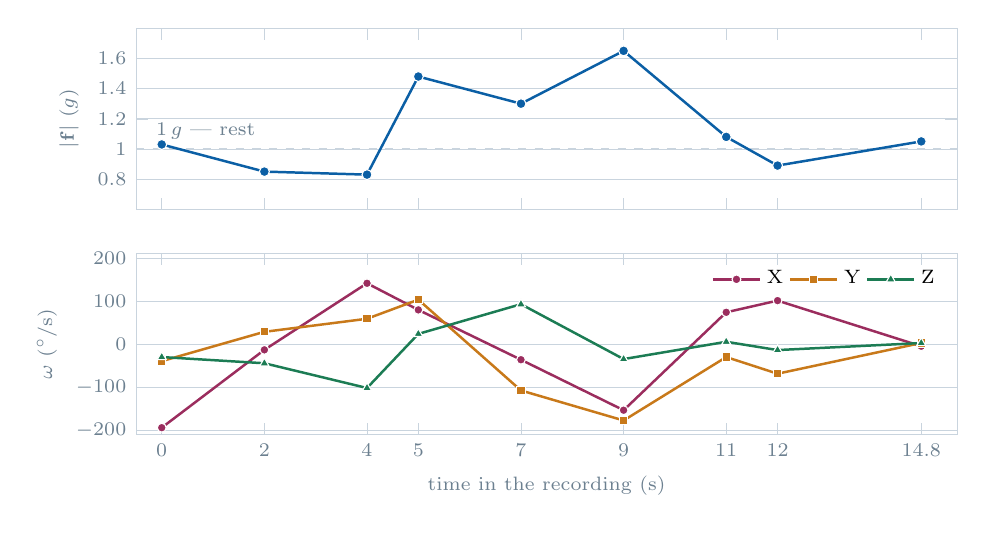
\begin{tikzpicture}
\begin{groupplot}[
  group style={group size=1 by 2, vertical sep=16pt, x descriptions at=edge bottom},
  width=0.86\textwidth, height=2.3cm, scale only axis,
  xmin=-0.5, xmax=15.5, xtick={0,2,4,5,7,9,11,12,14.8},
  xticklabels={0,2,4,5,7,9,11,12,14.8},
  tick label style={font=\scriptsize, color=cmnt},
  axis line style={rule, line width=0.4pt}, tick style={rule},
  ymajorgrids, grid style={rule, line width=0.3pt},
  ylabel style={font=\scriptsize, color=cmnt},
  xlabel={time in the recording (s)}, xlabel style={font=\scriptsize, color=cmnt},
  legend style={font=\scriptsize, draw=none, fill=none, at={(0.99,0.97)}, anchor=north east, legend columns=3},
  clip=false]
\nextgroupplot[ymin=0.6, ymax=1.8, ytick={0.8,1.0,1.2,1.4,1.6}, ylabel={$|\mathbf f|$ ($g$)}]
\addplot[rule, dashed, line width=0.6pt, forget plot] coordinates {(-0.5,1) (15.5,1)};
\addplot[accent, line width=0.9pt, mark=*, mark size=1.8pt, mark options={fill=accent, draw=white, line width=0.4pt}]
  coordinates {(0,1.03) (2,0.85) (4,0.83) (5,1.48) (7,1.30) (9,1.65) (11,1.08) (12,0.89) (14.8,1.05)};
\node[anchor=south west, font=\scriptsize, text=cmnt] at (axis cs:-0.3,1.0) {$1\,g$ --- rest};
\nextgroupplot[ymin=-210, ymax=210, ytick={-200,-100,0,100,200}, ylabel={$\omega$ ($^{\circ}$/s)}]
\addplot[num, line width=0.9pt, mark=*, mark size=1.6pt, mark options={fill=num, draw=white, line width=0.4pt}]
  coordinates {(0,-193.7) (2,-13.2) (4,141.2) (5,79.5) (7,-36.1) (9,-153.2) (11,73.9) (12,101.0) (14.8,-4.8)};
\addlegendentry{X}
\addplot[amber, line width=0.9pt, mark=square*, mark size=1.5pt, mark options={fill=amber, draw=white, line width=0.4pt}]
  coordinates {(0,-39.4) (2,28.6) (4,58.9) (5,103.2) (7,-107.4) (9,-177.0) (11,-29.9) (12,-68.5) (14.8,2.7)};
\addlegendentry{Y}
\addplot[str, line width=0.9pt, mark=triangle*, mark size=1.9pt, mark options={fill=str, draw=white, line width=0.4pt}]
  coordinates {(0,-29.9) (2,-44.3) (4,-101.7) (5,23.8) (7,92.7) (9,-34.6) (11,5.5) (12,-13.7) (14.8,2.6)};
\addlegendentry{Z}
\end{groupplot}
\end{tikzpicture}
\caption{The Part B readings over the recording. \emph{Top:} the magnitude of the
accelerometer vector sits at $1\,g$ at the start and end, when the sensor is still, and
swings away from it while the sensor is being moved --- the difference is the sensor's
own acceleration. \emph{Bottom:} the three gyroscope rates, large and changing sign
while the sensor is turned by hand, all within $\pm5\,^{\circ}$/s once it is set down.}
\label{fig:esp-trend}
\end{figure}

\begin{figure}[H]
\centering
\begin{minipage}[t]{0.32\textwidth}
\centering
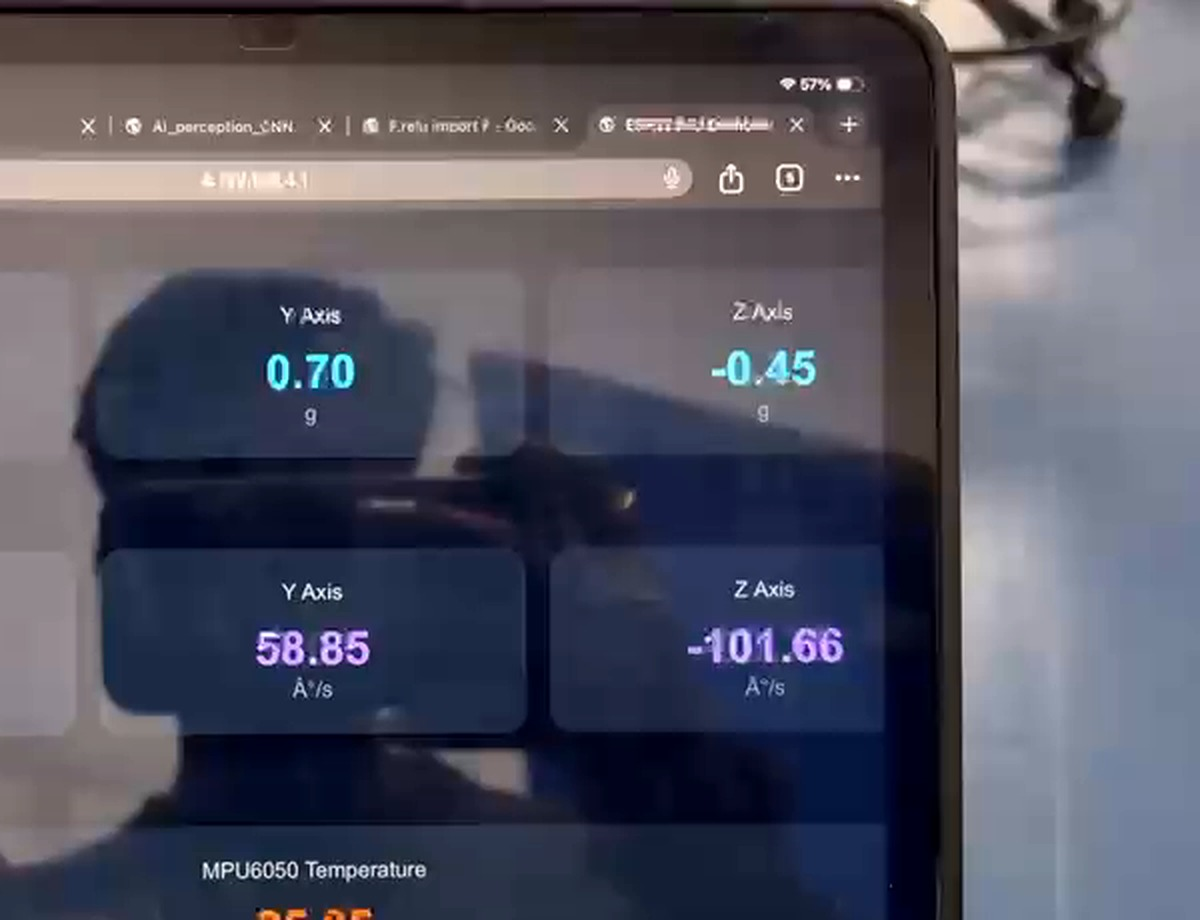
\includegraphics[width=\linewidth]{figures/esp32_imu_dashboard_a.jpg}\\[2pt]
{\scriptsize\color{cmnt} $t = 4\,$s, being tilted}
\end{minipage}\hfill
\begin{minipage}[t]{0.32\textwidth}
\centering
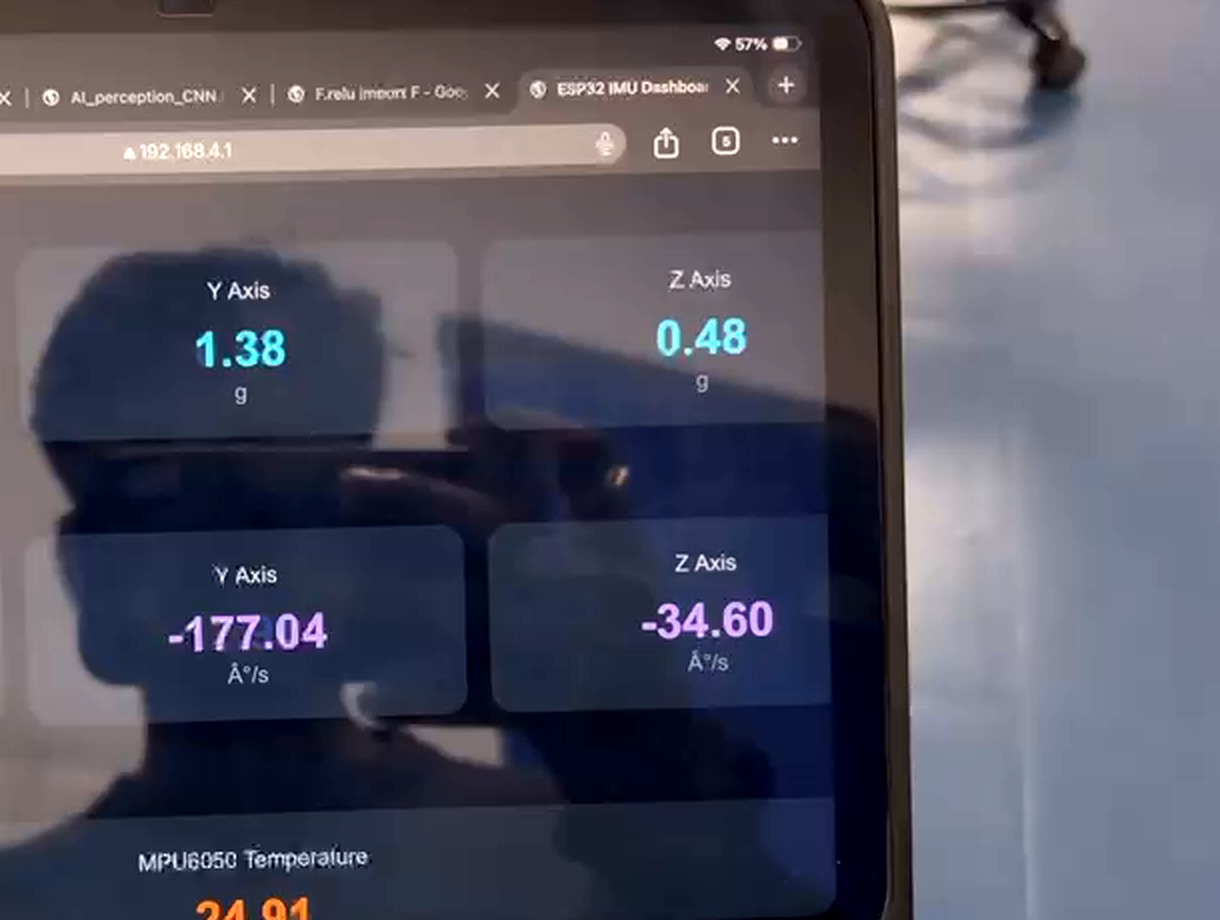
\includegraphics[width=\linewidth]{figures/esp32_imu_dashboard_b.jpg}\\[2pt]
{\scriptsize\color{cmnt} $t = 9\,$s, fastest movement}
\end{minipage}\hfill
\begin{minipage}[t]{0.32\textwidth}
\centering
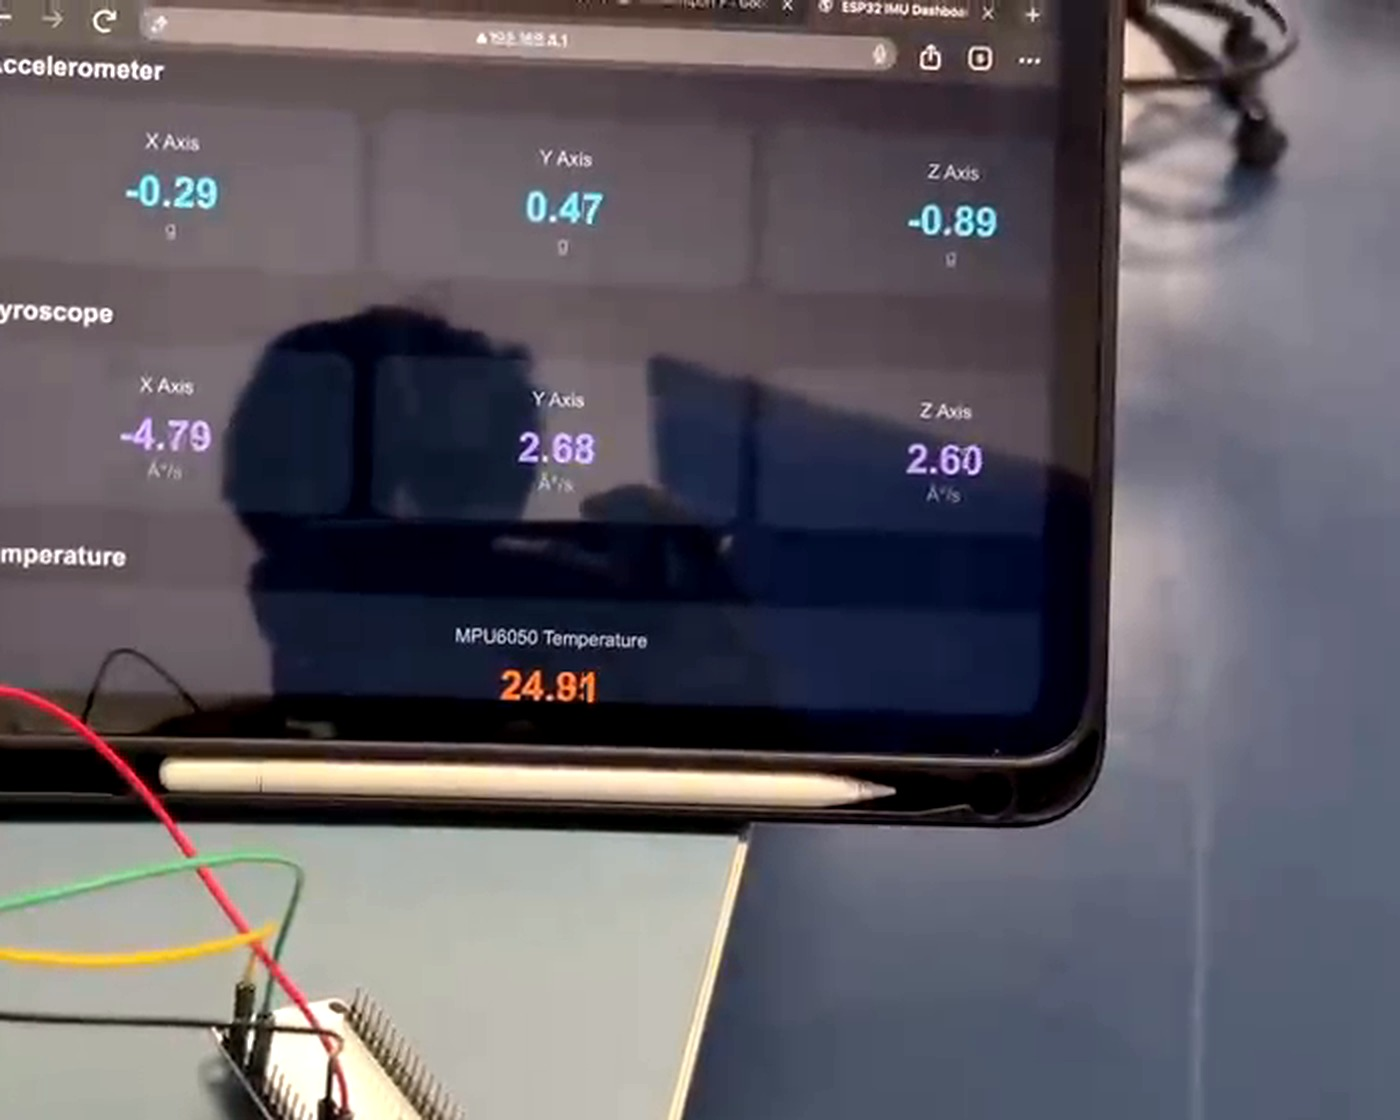
\includegraphics[width=\linewidth]{figures/esp32_imu_dashboard_c.jpg}\\[2pt]
{\scriptsize\color{cmnt} $t = 14.8\,$s, at rest}
\end{minipage}
\caption{Part B. The ``ESP32 IMU Dashboard'' served at \texttt{192.168.4.1}, viewed on
a tablet: three accelerometer cards in $g$, three gyroscope cards in $^{\circ}$/s and
the chip temperature. In the last frame the sensor has been set down: the gyroscope
is near zero and the accelerometer shows the $1\,g$ of gravity split over the axes by
the tilt of the desk-top module. (The ``\^{A}'' before the units is the same
encoding slip as in Experiment~5, fixed in Listing~\ref{lst:esp} by declaring the
charset.)}
\label{fig:dashboard}
\end{figure}

\subsection*{Checking the rest reading against the theory}

For the final frame, $(a_x, a_y, a_z) = (-0.29, 0.47, -0.89)\,g$:
\[
  |\mathbf f| = \sqrt{0.29^2 + 0.47^2 + 0.89^2} = 1.05\,g,\quad
  \text{pitch} = \arctan\frac{-0.29}{\sqrt{0.47^2+0.89^2}} = -16^{\circ},\quad
  \text{roll} = \arctan\frac{0.47}{\sqrt{0.29^2+0.89^2}} = 27^{\circ}.
\]
The magnitude is $1\,g$ to within the $\pm5\,\%$ that the uncalibrated $\pm2\,g$ range
of the MPU6050 typically gives, so the sensor was indeed at rest, resting at a tilt of
about $16^{\circ}$ and $27^{\circ}$ about its two horizontal axes --- it was lying on the
bundle of jumper wires, not flat. The gyroscope's $-4.8$, $2.7$ and $2.6\,^{\circ}$/s
are its zero-rate offsets, which a real application measures at start-up and subtracts.

\subsection*{Observed outputs --- Part A, Raspberry Pi terminal}

\vspace{2pt}
\noindent
{\small
\begin{tabularx}{\textwidth}{@{}c r r r r r r c c c c c c >{\centering\arraybackslash}X@{}}
\toprule
\rowcolor{soft}
\textbf{\#} & \multicolumn{3}{c}{\textbf{Accel (raw)}} & \multicolumn{3}{c}{\textbf{Gyro (raw)}} & \multicolumn{3}{c}{\textbf{Accel ($g$)}} & $|\mathbf f|$ & \multicolumn{3}{c}{\textbf{Gyro ($^{\circ}$/s)}} \\
\rowcolor{soft}
 & X & Y & Z & X & Y & Z & X & Y & Z & ($g$) & X & Y & Z \\
\midrule
1 & 7336 & -5528 & 14104 & -136 & 286 & 336 & $0.448$ & $-0.337$ & $0.861$ & 1.027 & $-1.0$ & $2.2$ & $2.6$ \\
2 & 7304 & -5660 & 14240 & -196 & 492 & 1 & $0.446$ & $-0.345$ & $0.869$ & 1.036 & $-1.5$ & $3.8$ & $0.0$ \\
3 & 7380 & -5732 & 14508 & -108 & 447 & 368 & $0.450$ & $-0.350$ & $0.885$ & 1.053 & $-0.8$ & $3.4$ & $2.8$ \\
4 & 7664 & -5588 & 14260 & -112 & 364 & -93 & $0.468$ & $-0.341$ & $0.870$ & 1.045 & $-0.9$ & $2.8$ & $-0.7$ \\
5 & 7424 & -5888 & 14168 & -106 & 353 & 141 & $0.453$ & $-0.359$ & $0.865$ & 1.040 & $-0.8$ & $2.7$ & $1.1$ \\
6 & 7348 & -5632 & 14332 & -38 & 132 & 31 & $0.448$ & $-0.344$ & $0.875$ & 1.041 & $-0.3$ & $1.0$ & $0.2$ \\
7 & 7336 & -5648 & 14096 & -104 & 259 & 223 & $0.448$ & $-0.345$ & $0.860$ & 1.029 & $-0.8$ & $2.0$ & $1.7$ \\
8 & 7348 & -5868 & 14180 & -120 & 443 & 247 & $0.448$ & $-0.358$ & $0.865$ & 1.038 & $-0.9$ & $3.4$ & $1.9$ \\
9 & 7360 & -5628 & 14280 & -98 & 386 & 118 & $0.449$ & $-0.344$ & $0.872$ & 1.039 & $-0.7$ & $2.9$ & $0.9$ \\
10 & 7332 & -5684 & 14336 & -206 & 416 & 152 & $0.448$ & $-0.347$ & $0.875$ & 1.042 & $-1.6$ & $3.2$ & $1.2$ \\
\bottomrule
\end{tabularx}}

\vspace{6pt}
\noindent Ten consecutive pairs of lines transcribed from the terminal
(Figure~\ref{fig:pi-terminal}); the module was resting on the desk throughout. The
raw counts are converted with $16384$ counts/$g$ and $131$ counts/($^{\circ}$/s). The
accelerometer values repeat to within about $\pm150$ counts ($\pm0.01\,g$), and the
magnitude is $1.039\,g$ on average --- the $1\,g$ of gravity to $3\,\%$. The
gyroscope reads $-0.9$, $2.7$ and $1.2\,^{\circ}$/s on average:
the zero-rate offsets of a sensor that is not turning, of the same size as those seen
at rest on the ESP32. From the mean acceleration $(0.451, -0.347, 0.870)\,g$
the module's attitude on the desk was pitch $26^{\circ}$ and roll
$-20^{\circ}$ --- it was lying on its jumper wires, tilted, as the
photograph in Figure~\ref{fig:pi-setup} shows.

\begin{figure}[H]
\centering
\begin{minipage}[t]{0.55\textwidth}
\vspace{0pt}
\centering
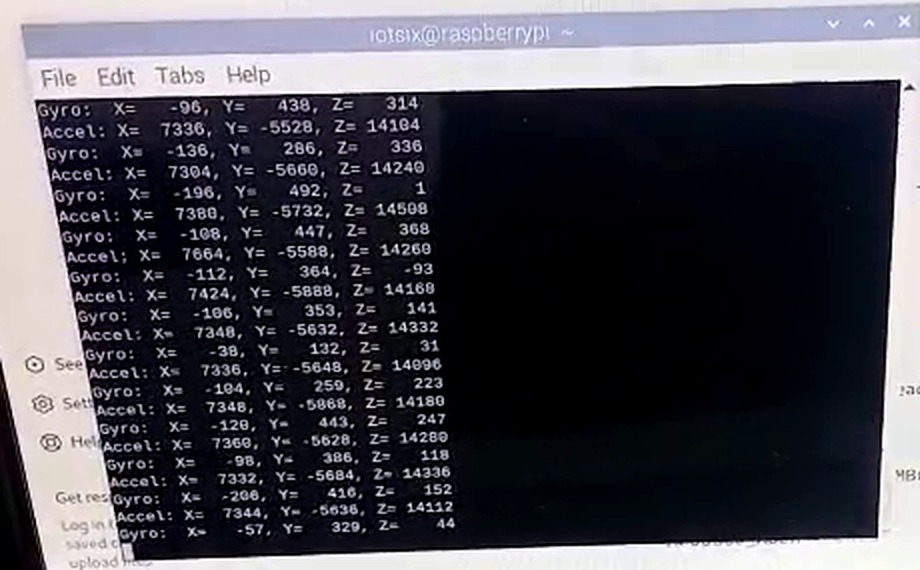
\includegraphics[width=\linewidth]{figures/rpi_imu_terminal.jpg}
\end{minipage}\hfill
\begin{minipage}[t]{0.43\textwidth}
\vspace{0pt}
\centering
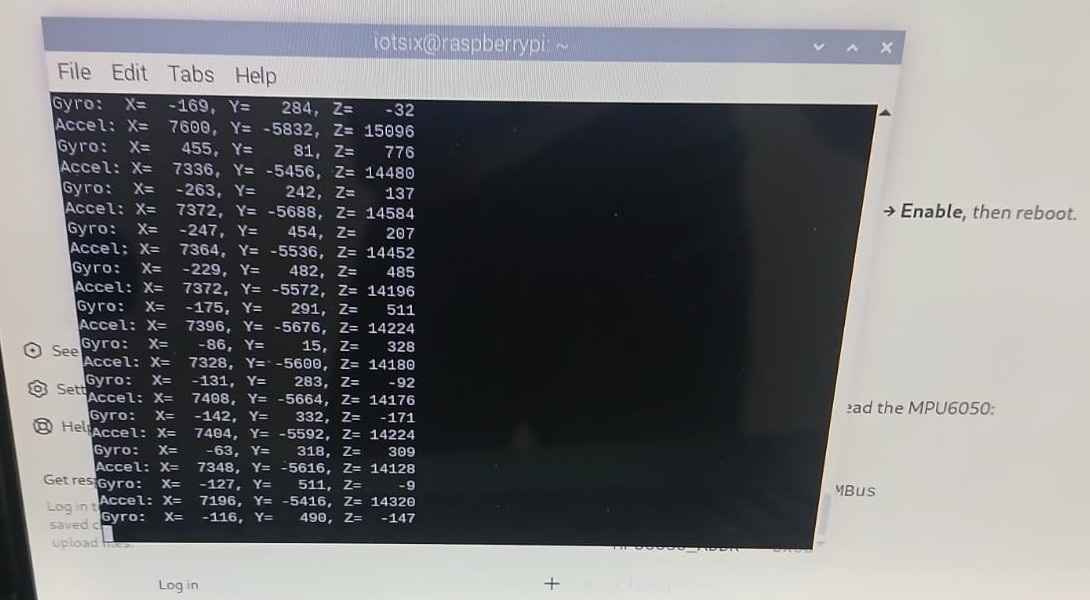
\includegraphics[width=\linewidth]{figures/rpi_imu_screen.jpg}
\end{minipage}
\caption{Part A on screen. \emph{Left:} the terminal while \texttt{imu.py} runs,
printing an \texttt{Accel} and a \texttt{Gyro} line of raw counts twice a second.
\emph{Right:} a wider view of the monitor: the terminal in front of the wiring notes
used for the setup (VCC $3.3\,\mathrm{V}$, GND, SDA $\to$ GPIO2 pin 3, SCL $\to$ GPIO3
pin 5).}
\label{fig:pi-terminal}
\end{figure}

\subsection*{The setups}

\begin{figure}[H]
\centering
\begin{minipage}[t]{0.42\textwidth}
\vspace{0pt}
\centering
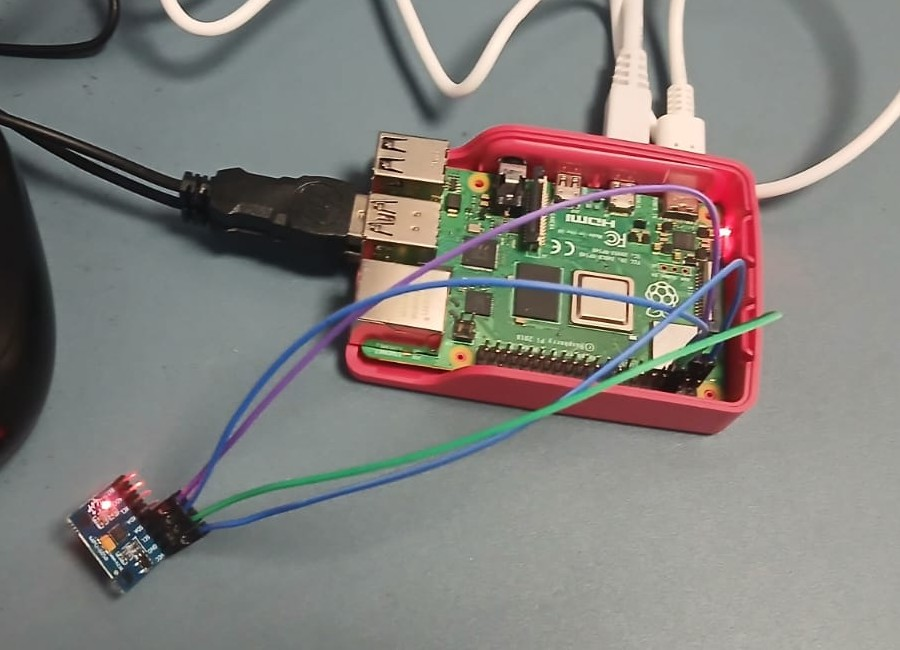
\includegraphics[width=\linewidth]{figures/rpi_mpu6050_setup.jpg}
\end{minipage}\hfill
\begin{minipage}[t]{0.42\textwidth}
\vspace{0pt}
\centering
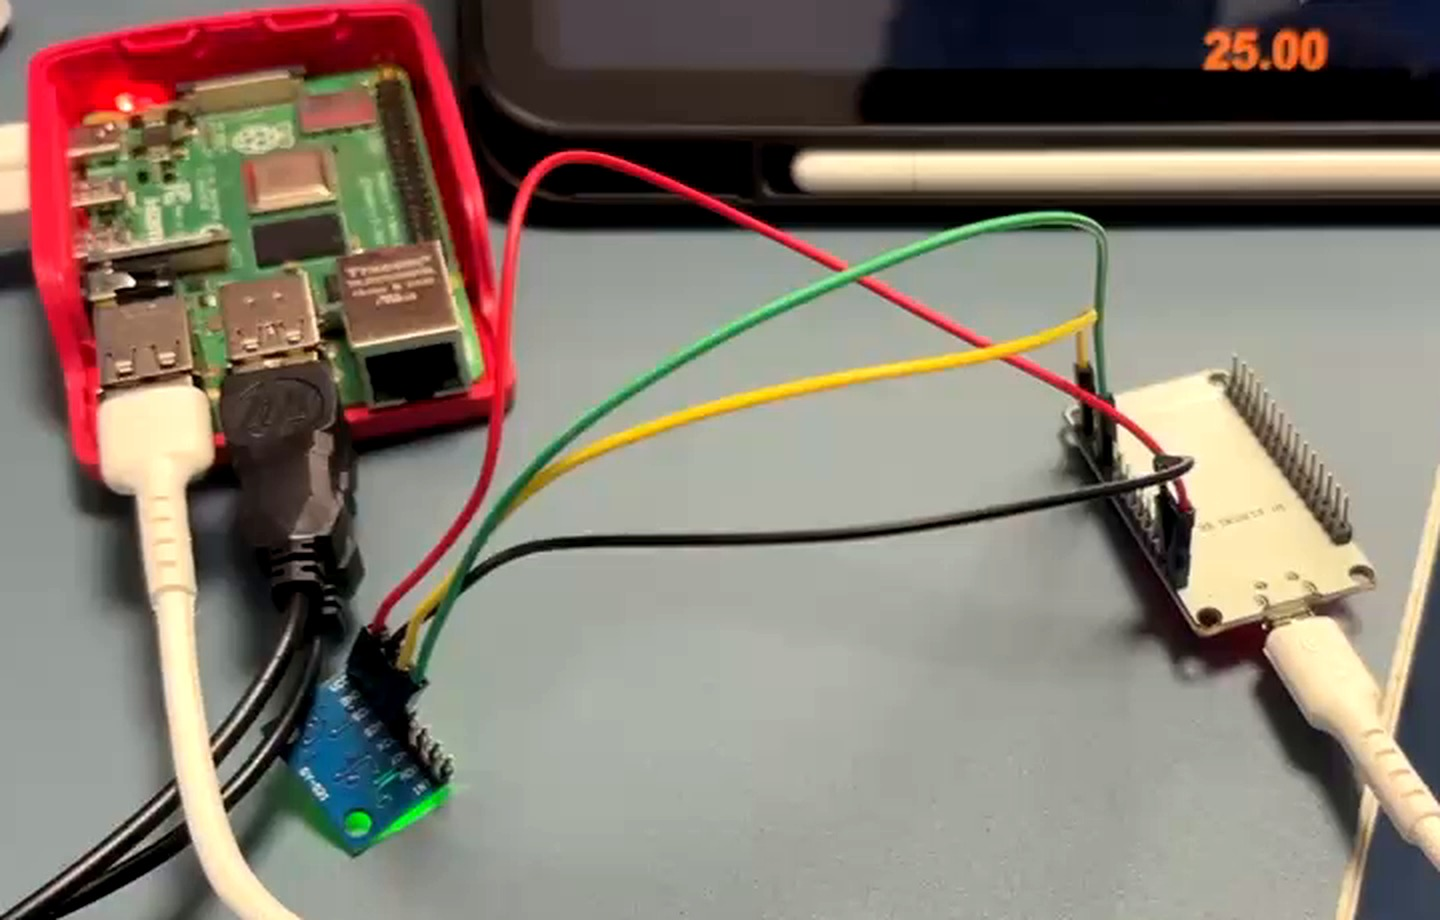
\includegraphics[width=\linewidth]{figures/esp32_mpu6050_wiring.jpg}
\end{minipage}\hfill
\begin{minipage}[t]{0.13\textwidth}
\vspace{0pt}
\centering
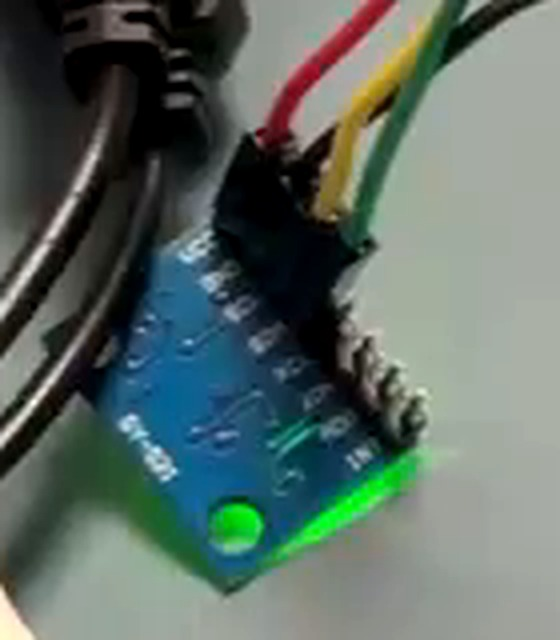
\includegraphics[width=\linewidth]{figures/gy521_module.jpg}
\end{minipage}
\caption{\emph{Left:} Part A --- the Raspberry Pi 4 with the GY-521 on four jumper
wires from the first rows of the header, the module lying tilted on the wires.
\emph{Centre:} Part B --- the ESP32 DevKit (powered from a USB port of the Pi) with the
same module --- red VCC, black GND, green SDA, yellow SCL --- in front of the tablet
showing the dashboard. \emph{Right:} the GY-521 with its power LED lit; the MPU6050
is the small square package in the centre.}
\label{fig:pi-setup}
\end{figure}

\subsection*{Video demonstration and code}

\begin{titledbox}[before skip=6pt]{Google Drive link}
\noindent The demonstration videos, this report and the complete source code are
available in the following shared folder:

\vspace{4pt}
\noindent\drivefolder

\vspace{4pt}
{\small\color{cmnt} Access has been set to \emph{anyone with the link can view}.}
\end{titledbox}

\subsection*{Discussion}
\label{sec:discussion}
\begin{itemize}
  \item \textbf{The accelerometer measures gravity too.} The clearest result of the
        experiment is that a motionless sensor reads $1\,g$, not zero. Only the
        \emph{deviation} of $|\mathbf f|$ from $1\,g$ in Figure~\ref{fig:esp-trend}
        --- down to $0.83\,g$ and up to $1.65\,g$ while the module was swung --- is the
        sensor's own acceleration, and separating the two properly needs the
        orientation from the gyroscope, exactly as the chain in Figure~\ref{fig:ins}
        shows.
  \item \textbf{Tilt from the accelerometer, turn rate from the gyroscope.} The
        rest readings on both boards gave the tilt of the module without any
        integration at all, because gravity is a fixed reference; the gyroscope, by
        contrast, only ever gives a \emph{rate}, and its reading returns to (nearly)
        zero the moment the motion stops. The two sensors are complementary: the
        accelerometer is drift-free but useless while the sensor is accelerating, the
        gyroscope is fast and unaffected by acceleration but drifts. Practical
        orientation filters (complementary or Kalman filters) blend them.
  \item \textbf{Why an IMU alone cannot navigate for long.} The residual gyroscope
        offsets of $2.6$--$4.8\,^{\circ}$/s at rest, if integrated, would rotate the
        estimated orientation by a full turn in under two minutes; the accelerometer's
        $5\,\%$ scale error, integrated twice, would place the sensor tens of metres away
        within a minute. Calibration at start-up (subtracting the zero-rate offsets,
        scaling $|\mathbf f|$ to exactly $1\,g$) reduces this, but not to zero, so
        inertial navigation always pairs the IMU with an external fix --- GPS or a
        barometer on the ground, star trackers and ground tracking on a spacecraft.
  \item \textbf{Sampling and filtering.} The dashboard refreshes five times a second,
        which is enough to watch but far too slow for navigation; the MPU6050 itself can
        deliver up to $1\,\mathrm{kHz}$ and has an on-chip low-pass filter
        (\texttt{setFilterBandwidth}) that trades noise for response time. A navigation
        loop would read it from a timer interrupt at a fixed rate, since the integrals
        depend on knowing $dt$ exactly.
  \item \textbf{Two ways to deliver the data.} As in Experiment~5, the Pi prints to a
        terminal while the ESP32 serves a web page from its own access point. The IMU
        shows the advantage of the second approach: with the sensor in the hand and the
        tablet on the desk, the live values could be watched while the module was
        moved, which a terminal on a fixed monitor made awkward.
\end{itemize}

%------------------------------------------------------------------ CONCLUSION
\Needspace{10\baselineskip}
\section{Conclusion}

The MPU6050 IMU was read over I$^2$C from both a Raspberry Pi and an ESP32, giving
three-axis acceleration and three-axis angular velocity in physical units. The Raspberry Pi
read the raw registers directly and showed a resting module at a steady $1.03\,g$ with
gyroscope offsets of a few $^{\circ}$/s; the ESP32 served the six values as a live
dashboard on its own Wi-Fi network, and its recording showed the behaviour the theory
predicts: a resting sensor reads a $1\,g$ acceleration
vector and a zero turn rate, tilting redistributes the $1\,g$ between the axes (from
which a tilt of $16^{\circ}$ and $27^{\circ}$ was recovered), and moving the sensor by hand
produced accelerations of up to $1.65\,g$ and turn rates of up to $180\,^{\circ}$/s.

These six quantities are the raw inputs of inertial navigation. The experiment also
showed its central difficulty: velocity, position and orientation are obtained by
integration, and the small biases seen at rest --- a few $^{\circ}$/s of gyroscope offset,
a few per cent of accelerometer scale --- grow without bound once integrated, which is
why an IMU is always used together with an absolute reference.

\end{document}
